%%%%%%%%%%%%%%%%%%%%%%%%%%%%%%%%%%%%%%%%%%%%%%%%%%%%%%%%%%%%
%2345678901234567890123456789012345678901234567890123456789012345678901234567890
%        1         2         3         4         5         6         7         8

%\documentclass[letterpaper, 10 pt, conference]{ieeeconf}  % Comment this line out
                                                          % if you need a4paper
\documentclass[a4paper, 10pt, conference]{ieeeconf}      % Use this line for a4
                                                          % paper

\IEEEoverridecommandlockouts                              % This command is only
                                                          % needed if you want to
                                                          % use the \thanks command
\overrideIEEEmargins
% See the \addtolength command later in the file to balance the column lengths
% on the last page of the document



% The following packages can be found on http:\\www.ctan.org
%\usepackage{graphics} % for pdf, bitmapped graphics files
%\usepackage{epsfig} % for postscript graphics files
%\usepackage{mathptmx} % assumes new font selection scheme installed
%\usepackage{times} % assumes new font selection scheme installed
%\usepackage{amsmath} % assumes amsmath package installed
%\usepackage{amssymb}  % assumes amsmath package installed
\usepackage{graphicx}

\title{\LARGE \bf
An  Industrial Robotic Knowledge Representation for Kit Building Applications\\
Title was: An OWL Ontology and Supporting SQL Database for Industrial Robotic Knowledge Representation
}

%\author{ \parbox{3 in}{\centering Huibert Kwakernaak*
%         \thanks{*Use the $\backslash$thanks command to put information here}\\
%         Faculty of Electrical Engineering, Mathematics and Computer Science\\
%         University of Twente\\
%         7500 AE Enschede, The Netherlands\\
%         {\tt\small h.kwakernaak@autsubmit.com}}
%         \hspace*{ 0.5 in}
%         \parbox{3 in}{ \centering Pradeep Misra**
%         \thanks{**The footnote marks may be inserted manually}\\
%        Department of Electrical Engineering \\
%         Wright State University\\
%         Dayton, OH 45435, USA\\
%         {\tt\small pmisra@cs.wright.edu}}
%}

\author{Author1 and Author2% <-this % stops a space
\thanks{This work was not supported by any organization}% <-this % stops a space
\thanks{H. Kwakernaak is with Faculty of Electrical Engineering, Mathematics and Computer Science,
        University of Twente, 7500 AE Enschede, The Netherlands
        {\tt\small h.kwakernaak@autsubmit.com}}%
\thanks{P. Misra is with the Department of Electrical Engineering, Wright State University,
        Dayton, OH 45435, USA
        {\tt\small pmisra@cs.wright.edu}}%
}


\begin{document}



\maketitle
\thispagestyle{empty}
\pagestyle{empty}


%%%%%%%%%%%%%%%%%%%%%%%%%%%%%%%%%%%%%%%%%%%%%%%%%%%%%%%%%%%%
\begin{abstract}

The IEEE RAS Ontologies for Robotics and Automation Working Group is dedicated to developing a methodology for knowledge representation and reasoning in robotics and automation. As part of this working group, the Industrial Robots sub-group is tasked with studying industrial applications of the ontology. One of the first areas of interest for this subgroup is in the area of kit building or kitting which is a process that brings parts together in a kit and then moves the kit to the assembly area where the parts are used in the final assembly. Kitting itself may be viewed as a specialization of the general bin-picking problem. This paper examines the knowledge representation that has been developed for the kitting problem and presents our real-time implementation of the knowledge representation along with a discussion of the trade-offs involved in its design.

\end{abstract}


%%%%%%%%%%%%%%%%%%%%%%%%%%%%%%%%%%%%%%%%%%%%%%%%%%%%%%%%%%%%
\section{INTRODUCTION}
Kitting is the process in which several different, but related items are placed into a container and supplied together as a single unit.
In industrial assembly of manufactured products, kitting is often performed prior to final assembly. Manufactures utilize kitting
due to its ability to provide cost savings \cite{Carlsson_2008} including saving manufacturing or assembly space \cite{Medbo2003}, reducing assembly workers walking and searching times \cite{Schwind1992}, and increasing line flexibility \cite{Bozer1992} and balance \cite{Jiao2000}.

Several different techniques are used to create kits. A kitting operation where a kit box is stationary until filled at a single
kitting workstation is refereed to as {\it batch kitting}. In {\it zone kitting}, the kit moves while being filled and will pass through one or
more zones before it is completed. This paper focuses on batch kitting processes.

In batch kitting, the kit's component parts may be staged in containers positioned in the workstation or may arrive on a conveyor.
Component parts may be fixtured, for example placed in compartments on trays, or may be in random orientations, for example
placed in a large bin. In addition to the kit's component parts, the workstation usually contains a storage area for empty kit boxes as
well as completed kits.

Kitting, has not yet been automated in many industries where automation may be feasible. Consequently, the cost of building kits is higher than it could be. We are addressing this problem by building models of the knowledge that will be required to operate an automated kitting workstation in an agile manufacturing environment. This workstation must be able to cope with
variations in kit contents, kit layout, and component supply. We also plan to develop a simulated kitting workstation for model validation. Our models
include representations for non-executable information about the workstation such as information about a robot, parts, kit designs, grippers, etc., models of executable information such as actions, preconditions, and effects, and models of the  process plan
necessary for kit construction. A discussion of the functional requirements for the process plan may be found in \cite{Balakirsky2012_1}.
For our automated kitting workstation, we assume that a robot performs a series of pick-and-place operations
in order to construct the kit. These operations include:
\begin{enumerate}
\item Pick empty kit and place on work table.
\item Pick multiple component parts and place in kit.
\item Pick completed kit and place in full kit storage area.
\end{enumerate}
Each of these actions may be a compound action that includes other actions such as end-of-arm tool changes, path planning,
and obstacle avoidance. 

It should be noted that multiple kits may be built simultaneously. Finished kits are moved to the assembly floor where components
are picked 
from the kit for use in the assembly procedure. The kits are normally designed to facilitate component picking in the correct
sequence for assembly. Component orientation may be constrained by the kit design in order to ease the pick-to-assembly process.
%The final kit does not normally contain small fasteners which are usually stored in the assembly area. 
Empty kits are returned to the kit building area for reuse.

Although the knowledge requirements described in the previous paragraph have been identified for the kitting domain, they are clearly applicable to many types of industrial robot applications (and likely to robot applications in other fields). As such, we expect that these knowledge requirements will serve as the basis for the industrial robot ontology being developed in the IEEE  RAS Ontologies for Robotics and Automation Working Group \cite{Madhavan2011} (hence forth referred to as the IEEE WG). Throughout the process of developing the kitting ontology, the group will constantly look at the applicability of the requirements outside of kitting and move the pertinent knowledge ``up'' the ontology (whether in the portion that models the kitting sub-domain, the industrials robot domain, or the upper ontology), as appropriate.

In keeping with our philosophy of producing standards in conjunction with the IEEE WG, we wish the models being developed by this effort to be as widely applicable as possible. To support this desire,we have
created a layered model abstraction where users may adopt as many or few of the layers of the abstraction as make sense for their
specific application.  The architecture shown in Figure \ref{fig:ProcessDataFlow}, though developed for the implementation of the kitting ontology, can be equally applicable to the implementation of any type of formal manufacturing knowledge representation. Said in a different way, the implementor can plug in a knowledge representation for a different domain and the architecture would still be valid. In a similar manner, different planning language abstractions could be utilized in the middle-layer of the 
abstraction and different planning/execution systems could be utilized in the top-layer of the abstraction. 

Specifics on the overall architecture may be found in Section \ref{sect:Architecture}. The lowest layer of the abstraction
is based on 
the Web Ontology Language (OWL) \cite{OWL} and is discussed further in Section \ref{sect:OWL_Layer}. The next layer of the 
abstraction is
modeled in the Planning Domain Definition Language (PDDL) \cite{PDDL}. More information on this layer may be found in Section
\ref{sect:PDDL_Layer}. In order to validate our models, we intend to utilize simulation in conjunction with  domain independent planning
systems and the Robot
Operating System (ROS) control environment \cite{ROS}. More information on this may be found in Section \ref{sect:ROS}. An example of the
various knowledge representations and the flow from one to the next is presented in Section \ref{sect:Example}. Finally,
conclusions and future work may be found in Section \ref{sect:Conclusions}.

%%%%%%%%%%%%%%%%%%%%%%%%%%%%%%%%%%%%%%%%%%%%%%%%%%%%%%%%%%%%
\begin{figure}[htb]
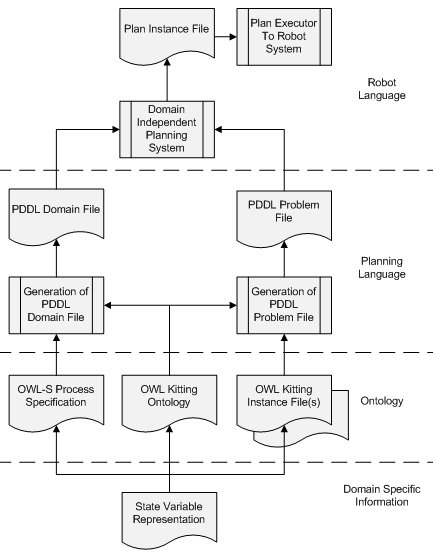
\includegraphics[width=7.6cm]{images/ProcessDataFlowV2.jpg}
\caption{Kitting data flow abstraction.}
\label{fig:ProcessDataFlow}
\end{figure}

\section{Architecture Description}
\label{sect:Architecture}
The main focus of this work is in the development of knowledge models that allow a kitting workstation to construct kits
in an agile manufacturing environment. However, in order to validate these knowledge models, we felt that it was
important to be able to utilize the models to construct kit building plans, and then to execute these plans in dynamic
virtual and real environments. Due to the advent of open source robotic operating systems such as ROS \cite{ROS} and simulation
packages such as USARSim \cite{Balakirsky2007} we do not need to design these systems ourselves. However, our architecture must
be designed to represent the required knowledge base in several different abstractions that are likely to be
required by these systems as the knowledge flows from process specification, to plan generation, to plan execution. 
As shown in Figure \ref{fig:ProcessDataFlow}, the abstraction is decomposed into three
distinct layers of {\it OWL Conformance}, {\it PDDL Conformance}, and {\it Robot Plan Conformance} that correspond to these
knowledge requirements. Implementors of the abstraction are free to utilize as many of the knowledge layers as make sense for
their particular application. For our simulated kitting workstation, we intend to fully design the OWL Conformance Layer and
then utilize open
source tools that will automatically generate the remaining layers and provide a workstation simulation.

\subsection{OWL Conformance}
``Ontology deals with questions concerning what entities exist or can be said to exist, and how such entities can be grouped, related within a hierarchy, and subdivided according to similarities and differences'' \cite{ontologyDef}.

Knowledge models may take many forms ranging from informal natural language, to XML schema, to ontologies. 
Since this work is being directed at the IEEE RAS Ontologies for Robotics and Automation Working Group, it is appropriate that our  knowledge representation be
encoded in an ontology at the lowest layer of our abstraction. The knowledge contained in this layer is sufficient for a planning system to understand the domain and construct
a plan for creating the desired kit from the given resources.

As shown in Figure \ref{fig:ProcessDataFlow} the information on our ontology is divided into three files and consists of a representation of the process specification,
the kitting ontology, and the instance file. The process specification file contains descriptions of
the individual actions and sequences necessary to construct a kit, e.g. gripping a component from a tray. The kitting ontology file contains the concepts related to the specific items 
that compose the kitting domain, e.g. a full description of each component including items such as the component's weight, dimensions, and grip points. The instance file
contains specific information on {\it this} particular kitting problem and configuration, e.g. component tray 1 contains 4 components of type `A'.

While this file set provides a complete description of the problem domain and environment, most planning systems cannot directly ingest information from an ontology.
Therefore, the second layer of the data abstraction known as the PDDL Conformance layer was created.

\subsection{PDDL Conformance}
By placing our knowledge in a domain independent representation, we enable the use of an entire family of open source planning systems. 
In particular, we have chosen to transform the information stored in the lower layer of our abstraction into the Planning Domain Definition Language (PDDL) \cite{PDDL}.
This provides our second layer of standardized output that other system may connect to. As shown in Figure \ref{fig:ProcessDataFlow}, this information consists of two files. The first
is a PDDL domain file that specifies all of the planning axioms and instances and is a summary of the process specification and ontology files. The second is a PDDL problem file that 
specifies the system's initial state and goal state. 

\subsection{Robot Plan Conformance}
The PDDL output may then be fed into a number of open source planning systems that will produce a plan instance file that is based on our original vocabulary. This file
contains a time sequenced series of actions that must be carried out in order to create a transition from our initial system state to the goal system state. Up to this point,
the entire architecture is independent of the kitting domain or any specific hardware configurations and is able to solve problems for many types of industrial robot applications. 
The top layer of our architecture ties the specific commands to the kitting workstation and is dependent on the workstation's resident hardware.  In order to maintain as
much hardware independence as possible, we have chosen to use the ROS environment for communicating with our simulation. Therefore, the PDDL commands will
be translated into appropriate commands that will be sent into various ROS processes.

%%%%%%%%%%%%%%%%%%%%%%%%%%%%%%%%%%%%%%%%%%%%%%%%%%%%%%%%%%%%
\section{OWL Model of Manufacturing Process}
\label{sect:OWL_Layer}
For the development of the  knowledge representation, the industrial robots sub-group has decided to use OWL (Web Ontology Language) \cite{OWL} as the knowledge representation language. OWL is a family of knowledge representation languages for authoring ontologies and is endorsed by the World Wide Web Consortium (W3C). It is characterized by formal semantics and RDF/XML-based serialization for the Semantic Web. OWL was chosen by the group because of its popularity among the ontology development community, its endorsement by the W3C, as well as the number of tools and reasoning engines that are available. OWL was also selected at the representation language that will be used in the overall IEEE WG efforts.

In addition to OWL, the industrial robots subgroup will also be using OWL-S \cite{Martin2012} to represent the processes and actions that the robot will perform. OWL-S is an ontology built on top of OWL by the DARPA Agent Markup Language (DAML) program \cite{damlWeb}
for describing Semantic Web Services. However, many of the constructs that are used to describe services are equally applicable to describing robot actions. For example, concepts such as preconditions, results, inputs, outputs, effects, and participants are generic enough to be applied to just about any type of process specification. 

To build the ontology, the group has taken a very systematic approach of identifying and modeling the concepts. Because the industrial robot field is so broad, the group decided to limit its efforts to a single type of operation, namely kitting. A scenario was developed that described, in detail, the types of operations that would be performed in kitting, the sequencing of steps, the parts and machines that were needed, constraints on the process such as pre- and post-conditions, etc. For this scenario, a set of concepts were extracted and defined. These concepts served as the initial requirements for the kitting ontology. The concepts were then modeling in OWL, building off of the definitions and relationships that were identified in the scenario. 

As more detailed scenarios are determined and a richer set of concepts are uncovered, the ontology will be partitioned based upon the generality of the concept, with the most generally applicable concepts being ``higher'' in the ontology so they are available to other domains and the more detailed concepts being ``lower'' in the ontology because they will likely be very specific to the kitting area. An example of a general concept may be a ``robot'' while a specific concept may be a ``kit box.''

Some of the concepts that are represented in the ontology include:
\begin{itemize}
\item	Gripper Effector - A GripperEffector is an EndEffector. A GripperEffector holds an object by gripping it with fingers or claws.
\item	KitTrays - A KitTray is designed to hold Parts with various SKU ids in known positions.
\item	KittingWorkStation - A KittingWorkstation contains a work table, a robot, an EndEffectorChangingStation (where various end-of-arm tooling is stored and attached/removed from the robot), and other fixed obstacles such as a computer. A KittingWorkstation has an angle unit, a length unit and a weight unit. All angle, length, and weight values related to the workstation must use those units. A KittingWorkstation has a list of Stock Keeping Units (SKUs) it knows about. In addition, containers of various sorts enter and leave the workstation.  The robot builds kits of parts by executing kitting plans as directed by a kitting plan execution system.
\item	Part - A Part has a reference to the identifier of a SKU and a Serial Number.
\item	PartsBin - A PartsBin holds a number of Parts with the same SKU id in unknown random positions, or fixtured known positions.
\item	Robot - A Robot has a description, a robot id, a work volume, an end effector, and a maximum load weight.
\item	VacuumEffector - A VacuumEffector holds an object by putting a cup against the object and applying a vacuum. It contains the maximum lifting force and the vacuum cup configuration.
\item	 WorkTable - The top of a WorkTable is a flat, rectangular, horizontal surface.
\end{itemize}


%%%%%%%%%%%%%%%%%%%%%%%%%%%%%%%%%%%%%%%%%%%%%%%%%%%%%%%%%%%%
\section{PDDL Model of Manufacturing Process}
\label{sect:PDDL_Layer}
%PDDL is a recent attempt to standardize planning domain and problem description languages. A state-variable representation (SVR)~\cite{NAU.2004} is used to define the planning domain and problem that will be translated in PDDL format. In a SVR, each state is represented by a tuple of values of $n$ state variables $\lbrace x_1,\dots,x_n\rbrace$, and each action is represented by a partial function that maps this tuple into some other tuple of values of the $n$ state variables.
%\subsection{Planning Domain for Kitting}

\subsection{Constant Symbols for the Kitting Domain}
In the SVR, constant symbols are partitioned into disjoint classes corresponding to the objects of the domain. For the kitting domain, these classes are derived from the concepts represented in the ontology (see Section~\ref{sect:OWL_Layer}). The finite set of all constant symbols in the kitting domain is partitioned into the following sets of constant symbols:
\begin{small}
\begin{itemize}
\item A set of \emph{robots}: a robot in the kitting workstation is a robotic arm that can move objects in order to build kits.

\item A set of \emph{kit trays}: kit trays are compartments that can hold parts. A kit is built when a kit tray contains all the parts necessary to produce a kit. A kit tray is empty when it does not contain any part and finished when it contains all the parts that constitute a kit. When a kit tray is neither empty nor finished, it is partially full.

\item A set of \emph{part bins}: parts are placed in part bins and each part bin contains one type of parts.

\item A set of \emph{parts}: parts are delivered to the workstation in part bins and are placed in kit trays.

\item A set of \emph{gripper effectors}: a gripper effector holds an object by gripping it with
fingers or claws.

\item A set of \emph{gripper effector holders}: a gripper effector holder holds one type of gripper effectors.

\item A symbol \emph{changing station}: a changing station is made up of gripper effector holders.

\item A set of \emph{boxes of finished kit trays}: a box that contains only finished kits.

\item A set of \emph{boxes of empty kit trays}: a box that contains only empty kit trays.

\item A symbol \emph{work table}: A work table is an area in the kitting workstation where kit trays are placed to build kits.
\end{itemize}
\end {small}
\subsection{State Variable Symbols for the Kitting Domain}
State variable symbols are functions from the set of states and zero or more sets of constant variables into a set of constant variables~\cite{NAU.2004}. Using state variable symbols reduces possibilities for inconsistent states and generates a smaller state space. A state variable symbol is an expression of the form ...The following state variable symbols are used in the kitting domain:
\begin{itemize}
\item geffloc: \emph{gripper effectors}$\times S\rightarrow$ \emph{robots} $\cup$ \emph{gripper effector holders}: designates the location of a gripper effector in the workstation. The gripper can be in a gripper effector holder or attached to the robot.


\item rgrip: \emph{robots}$\times S\rightarrow$\emph{gripper effectors} $\cup$ $\lbrace nil\rbrace$: designates the gripper effector that is attached to a robot or $nil$ if no gripper effector is attached.

\item topworktable: \emph{work table} $\times S \rightarrow$ \emph{kit trays} $\cup$ $\lbrace nil\rbrace$: designates the object placed on the work table: a kit tray or nothing ($nil$).

\item \texttt{ktloc}: \emph{kit trays} $\times S \rightarrow$ \emph{boxes of empty kit trays} $\cup$ \emph{boxes of finished kit trays} $\cup$ \emph{work table} $\cup$ \emph{robots}: designates the different possible locations of a kit tray in the workstation. The kit tray can be in the box of empty kit trays, in the box of finished kit trays, on the work table, or in the robot's gripper effector.

\item \texttt{ploc}: \emph{parts} $\times S \rightarrow$ \emph{part bins} $\cup$ \emph{kit trays} $\cup$ \emph{robots}: designates the different possible locations of a part in the workstation. The part can be in a part bin, in a kit tray, or in the robot's gripper effector.

\item \texttt{rhold}: \textit{robots} $\times S \rightarrow$ \textit{kit trays} $\cup$ \textit{parts} $\cup$ $\lbrace nil\rbrace$: designates the object being held by the robot. It can be a kit tray, a part, or nothing ($nil$). It is assumed that the robot is already equipped with the appropriate gripper effector.

\item \texttt{isboxfktfull}: \textit{boxes of finished kit trays} $\times$ $S \rightarrow$ $\lbrace 0\rbrace$ $\cup$ $\lbrace 1\rbrace$: designates if a box of finished kit trays is full (1) or not (0).

\item \texttt{isboxektempty}: \textit{boxes of empty kit trays} $\times$ $S \rightarrow$ $\lbrace 0\rbrace$ $\cup$ $\lbrace 1\rbrace$: designates if a box of empty kit trays is empty (1) or not (0).

\item \texttt{ispartbinempty}: \textit{part bins} $\times$ $S \rightarrow$ $\lbrace 0\rbrace$ $\cup$ $\lbrace 1\rbrace$: designates if a part bin is empty (1) or not (0).

\item \texttt{gefftype}: \textit{gripper effectors} $\times$ $S \rightarrow$ \textit{kit trays} $\cup$ \textit{parts}: designates the type of object the gripper effector can hold. For the kitting domain used in this paper, a gripper effector can hold two types of object: kit trays and parts.
\end{itemize}

%\subsection{Planning Problem for Kitting}

\subsection{Planning Operators for Kitting}
A planning operator~\cite{NAU.2004} is a triple \textit{o=(name(o), precond(o), effects(o))}
where:
\begin{itemize}
\item name(o) is a syntactic expression of the form $n(u_1,\dots,u_k)$, where $n$ is a symbol
called an operator symbol, $u_1,\dots,u_k$ are all of the object variable symbols that
appear anywhere in \textit{o}, and $n$ is unique (i.e., no two operators can have the
same operator symbol).
\item precond(o) is a set of expressions on state variables and relations.
\item effects(o) is a set of assignments of values to state variables of the form
$x(t_1,\dots,t_k)\leftarrow t_{k+1}$, where each $t_i$ is a term in the appropriate range.
\end{itemize}

The kitting domain is constituted of the eight following operators:
\begin{small}
\begin{enumerate}
\item \textsl{take-kt-bekt} ($\mathrm{r}$, $\mathrm{kt}$, $\mathrm{boxekt}$, $\mathrm{geff}$)
\begin{itemize}
\item ;;The robot $\mathrm{r}$ is equipped with the gripper effector $\mathrm{geff}$ to pick up the kit tray $\mathrm{kt}$ from the box of empty kit trays $\mathrm{boxekt}$.
\item precond:
\begin{itemize}
\item[]\emph{ktloc}$\mathrm{(kt)=boxekt}$
\item[]\emph{rhold}$\mathrm{(r)=nil}$
\item[]\emph{rgrip}$\mathrm{(r)=geff}$
\item[]\emph{isboxektempty}$\mathrm{(kt)=0}$
\item[]\emph{geffloc}$\mathrm{(geff)=r}$
\end{itemize}
\item effects:
\begin{itemize}
\item[]\emph{ktloc}$\mathrm{(kt)\leftarrow r}$
\item[]\emph{rhold}$\mathrm{(r)\leftarrow kt}$
\end{itemize}
\end{itemize}

\item \textsl{put-kt-wtable} ($\mathrm{r}$, $\mathrm{kt}$, $\mathrm{wtable}$)
\begin{itemize}
\item ;;The robot $\mathrm{r}$ puts down the kit tray $\mathrm{kt}$ on the work table $\mathrm{wtable}$.
\item precond:
\begin{itemize}
\item[]\emph{ktloc}$\mathrm{(kt)=r}$
\item[]\emph{rhold}$\mathrm{(r)=kt}$
\item[]\emph{topworktable}$\mathrm{(wtable)=nil}$
\end{itemize}
\item effects:
\begin{itemize}
\item[]\emph{ktloc}$\mathrm{(kt)\leftarrow wtable}$
\item[]\emph{rhold}$\mathrm{(r)\leftarrow nil}$
\item[]\emph{topworktable}$\mathrm{(r)\leftarrow kt}$
\end{itemize}
\end{itemize}

\item \textsl{take-kt-wtable} ($\mathrm{r}$, $\mathrm{kt}$, $\mathrm{wtable}$, $\mathrm{geff}$)
\begin{itemize}
\item ;;The robot $\mathrm{r}$ picks up the kit tray $\mathrm{kt}$ from the work table $\mathrm{wtable}$.
\item precond:
\begin{itemize}
\item[]\emph{ktloc}$\mathrm{(kt)=wtable}$
\item[]\emph{rhold}$\mathrm{(r)=nil}$
\item[]\emph{topworktable}$\mathrm{(wtable)=kt}$
\item[]\emph{rgrip}$\mathrm{(r)=geff}$
\item[]\emph{geffloc}$\mathrm{(geff)=r}$
\end{itemize}
\item effects:
\begin{itemize}
\item[]\emph{ktloc}$\mathrm{(kt)\leftarrow nil}$
\item[]\emph{rhold}$\mathrm{(r)\leftarrow kt}$
\item[]\emph{topworktable}$\mathrm{(r)\leftarrow nil}$
\end{itemize}
\end{itemize}

\item \textsl{put-kt-bfkt} ($\mathrm{r}$, $\mathrm{kt}$, $\mathrm{boxfkt}$)
\begin{itemize}
\item ;;The robot $\mathrm{r}$ puts down the kit tray $\mathrm{kt}$ in the box of finished kit trays $\mathrm{boxfkt}$.
\item precond:
\begin{itemize}
\item[]\emph{ktloc}$\mathrm{(kt)=nil}$
\item[]\emph{rhold}$\mathrm{(r)=kt}$
\item[]\emph{isboxfktfull}$\mathrm{(boxfkt)=0}$
\end{itemize}
\item effects:
\begin{itemize}
\item[]\emph{ktloc}$\mathrm{(kt)\leftarrow boxfkt}$
\item[]\emph{rhold}$\mathrm{(r)\leftarrow nil}$
\end{itemize}
\end{itemize}

\item \textsl{take-p} ($\mathrm{r}$, $\mathrm{p}$, $\mathrm{pb}$, $\mathrm{geff}$)
\begin{itemize}
\item ;;Robot $\mathrm{r}$ uses gripper effector $\mathrm{geff}$ to pick up part $\mathrm{p}$ from part bin $\mathrm{pb}$.
\item precond:
\begin{itemize}
\item[]\emph{ploc}$\mathrm{(p)=pb}$
\item[]\emph{rhold}$\mathrm{(r)=nil}$
\item[]\emph{rgrip}$\mathrm{(r)=geff}$
\item[]\emph{ispartbinempty}$\mathrm{(pb)=0}$
\item[]\emph{geffloc}$\mathrm{(geff)=r}$

\end{itemize}
\item effects:
\begin{itemize}
\item[]\emph{ploc}$\mathrm{(p)=r}$
\item[]\emph{rhold}$\mathrm{(r)=p}$
\end{itemize}
\end{itemize}

\item \textsl{put-p} ($\mathrm{r}$, $\mathrm{p}$, $\mathrm{kt}$)
\begin{itemize}
\item ;;Robot $\mathrm{r}$ puts down part $\mathrm{p}$ in kit tray $\mathrm{kt}$.
\item precond:
\begin{itemize}
\item[]\emph{ploc}$\mathrm{(p)=r}$
\item[]\emph{rhold}$\mathrm{(r)=p}$
\end{itemize}
\item effects:
\begin{itemize}
\item[]\emph{ploc}$\mathrm{(p)=kt}$
\item[]\emph{rhold}$\mathrm{(r)=nil}$
\end{itemize}
\end{itemize}

\item \textsl{attach-geff} ($\mathrm{r}$, $\mathrm{geff}$, $\mathrm{geffholder}$)
\begin{itemize}
\item ;;Robot $\mathrm{r}$ attaches gripper effector $\mathrm{geff}$ from gripper effector holder $\mathrm{geffholder}$.
\item precond:
\begin{itemize}
\item[]\emph{geffloc}$\mathrm{(geff)=geffholder}$
\item[]\emph{rgrip}$\mathrm{(r)=nil}$
\end{itemize}
\item effects:
\begin{itemize}
\item[]\emph{geffloc}$\mathrm{(geff)=r}$
\item[]\emph{rgrip}$\mathrm{(r)=geff}$
\end{itemize}
\end{itemize}

\item \textsl{remove-geff} ($\mathrm{r}$, $\mathrm{geff}$, $\mathrm{geffholder}$)
\begin{itemize}
\item ;;Robot $\mathrm{r}$ removes gripper effector $\mathrm{geff}$ and put it in gripper effector holder $\mathrm{geffholder}$.
\item precond:
\begin{itemize}
\item[]\emph{geffloc}$\mathrm{(geff)=r}$
\item[]\emph{rgrip}$\mathrm{(r)=geff}$
\end{itemize}
\item effects:
\begin{itemize}
\item[]\emph{geffloc}$\mathrm{(geff)=geffholder}$
\item[]\emph{rgrip}$\mathrm{(r)=nil}$
\end{itemize}
\end{itemize}
\end{enumerate}
\end{small}


\begin{comment}
\begin{tabular}{p{3.5cm}p{3.5cm}}
\begin{itemize}
\item[]\emph{ktloc}$\mathrm{(kt)\leftarrow nil}$
\item[]\emph{rhold}$\mathrm{(r)\leftarrow kt}$
\item[]\emph{topworktable}$\mathrm{(r)\leftarrow nil}$
\end{itemize} & \begin{itemize}
\item[]\emph{ktloc}$\mathrm{(kt)\leftarrow nil}$
\item[]\emph{rhold}$\mathrm{(r)\leftarrow kt}$
\item[]\emph{topworktable}$\mathrm{(r)\leftarrow nil}$
\end{itemize}
\end{tabular}

\begin{table}[ht]
\centering
\begin{tabular}{|c|p{6cm}|} \hline
\multirow{4}{*}{\begin{sideways}{\small \textsl{take-kt-bekt}}\end{sideways}} & \rule[-1ex]{0pt}{3.5ex} {\small $\mathrm{r}$, $\mathrm{kt}$, $\mathrm{boxekt}$, $\mathrm{geff}$}  \T\\ \cline{2-2}
&\rule[-1ex]{0pt}{3.5ex}{\small The robot $\mathrm{r}$ is equipped with the gripper effector $\mathrm{geff}$ to pick up the kit tray $\mathrm{kt}$ from the box of empty kit trays $\mathrm{boxekt}$.}\T \\ \cline{2-2}
& {\small \emph{ktloc}($\mathrm{kt}$)$\mathrm{= boxekt}$, \emph{rhold}($\mathrm{r}$)$\mathrm{= nil}$, \emph{rgrip}($\mathrm{r}$)$\mathrm{= geff}$, \emph{isboxektempty}($\mathrm{kt}$)$=0$} \\
& Max-Min \\ \hline
\end{tabular}
\end{table}


The operators on the kitting domain are defined as follows:

\begin{itemize}
\item \textbf{take\_kt\_bekt} (\emph{r}, \emph{kt}, \emph{boxekt})
\begin{itemize}
\item ;;The robot \emph{r} takes the kit tray \emph{kt} from the box of empty kit trays \emph{boxekt}.
\item \textit{precond}: \textit{ktloc}(\ekt)=\boxekt, \textit{rhold}(\robot)=\nil
\item \textit{effects}: \textit{ektloc}(ekt)=\robot, \textit{rhold}(\robot)=\ekt
\end{itemize}

\item \textit{putEkt} (\robot, \ekt, \wtable)
\begin{itemize}
\item ;;The robot \robot puts the empty kit tray \ekt on the work table \wtable.
\item \textit{precond}: \textit{ektloc}(\ekt)=\robot, \textit{rhold}(\robot)=\ekt
\item \textit{effects}: \textit{ektloc}(\ekt)=\wtable, \textit{rhold}(\robot)=\nil
\end{itemize}

\item \textit{takeFkt} (\robot, \fkt, \wtable)
\begin{itemize}
\item ;;The robot \robot takes the full kit tray \fkt from the work table \wtable.
\item \textit{precond}: \textit{fktloc}(\fkt)=\wtable, \textit{rhold}(\robot)=\nil
\item \textit{effects}: \textit{fktloc}(\fkt)=\robot, \textit{rhold}(\robot)=\fkt
\end{itemize}

\item \textit{putFkt} (\robot, \fkt, \boxekt)
\begin{itemize}
\item ;;The robot \robot puts the full kit tray \fkt in the box of full kit trays \boxfkt.
\item \textit{precond}: \textit{ektloc}(\fkt)=\robot, \textit{rhold}(\robot)=\fkt
\item \textit{effects}: \textit{ektloc}(\fkt)=\boxfkt, \textit{rhold}(\robot)=\nil
\end{itemize}

\item \textit{takeP} (\robot, \parts, \partsup)
\begin{itemize}
\item ;;The robot \robot takes the part \parts from the part supply tray \partsup.
\item \textit{precond}: \textit{ploc}(\parts)=\partsup, \textit{rhold}(\robot)=\nil
\item \textit{effects}: \textit{ploc}(\parts)=\robot, \textit{rhold}(\robot)=\parts
\end{itemize}

\item \textit{putP} (\robot, \parts, \kt)
\begin{itemize}
\item ;;The robot \robot puts the part \parts in the kit tray \kt.
\item \textit{precond}: \textit{ploc}(\parts)=\robot, \textit{rhold}(\robot)=\parts
\item \textit{effects}: \textit{ploc}(\parts)=\kt, \textit{rhold}(\robot)=\nil
\end{itemize}

\item \textit{aboveP} (\parts, {\constant{pos1}}, {\constant{pos2}})
\begin{itemize}
\item ;;The robot r stations over the part \parts at the position pos2. The previous position of the robot is pos1.
\item \textit{precond}: \textit{rpos}(\robot)={\constant{pos1}}
\item \textit{effects}: \textit{rpos}(\robot)={\constant{pos2}}
\end{itemize}

\item \textit{aboveKit} (\kt, {\constant{pos1}}, {\constant{pos2}})
\begin{itemize}
\item ;;The robot \robot stations over the kit tray \kt at the position pos2. The previous position of the robot is pos1.
\item \textit{precond}: \textit{rpos}(\robot)={\constant{pos1}}
\item \textit{effects}: \textit{rpos}(\robot)={\constant{pos2}}
\end{itemize}

\item \textit{aboveBekt} (\boxekt, {\constant{pos1}}, {\constant{pos2}})
\begin{itemize}
\item ;;The robot \robot stations over the box of empty kit trays at the position pos2. The previous position of the robot is pos1.
\item \textit{precond}: \textit{rpos}(\robot)={\constant{pos1}}
\item \textit{effects}: \textit{rpos}(\robot)={\constant{pos2}}
\end{itemize}

\item \textit{aboveBfkt} (\boxfkt, {\constant{pos1}}, {\constant{pos2}})
\begin{itemize}
\item ;;The robot \robot stations over the box of full kit trays at the position {\constant{pos2}}. The previous position of the robot is {\constant{pos1}}, the final position is {\constant{pos2}}.
\item \textit{precond}: \textit{rpos}(\robot)={\constant{pos1}}
\item \textit{effects}: \textit{rpos}(\robot)={\constant{pos2}}
\end{itemize}

\item \textit{attach} (\robot, \grip, \chstation)
\begin{itemize}
\item ;;The robot \robot attaches the gripper \grip.
\item \textit{precond}: \textit{gloc}(\grip)=chstation,
\item \textit{effects}: \textit{gloc}(\grip)=\robot
\end{itemize}

\item \textit{remove} (\robot, \grip, chstation)
\begin{itemize}
\item ;;The robot \robot removes the gripper \grip.
\item \textit{precond}: \textit{gloc}(\grip)=\robot,
\item \textit{effects}: \textit{gloc}(\grip)=\chstation
\end{itemize}
\end{itemize}
\end{comment}

\subsubsection{Definition of the Initial State}

\subsubsection{Definition of the Goal State}


%%%%%%%%%%%%%%%%%%%%%%%%%%%%%%%%%%%%%%%%%%%%%%%%%%%%%%%%%%%%
\section{ROS Model of Manufacturing Process}
\label{sect:ROS}
When developing a knowledge representation, it is very difficult to determine if the representation is sufficient for actual use in a dynamic, unstructured environment.
One technique that may be utilized that provides repeatable experiments with deterministic amounts of noise and world variance is simulation. As part of our kitting work
station implementation, we are developing an open source application that will translate our PDDL command syntax into standard ROS topics for the ROS Arm Navigation 
Stack known as arm\_navigation.

%%%%%%%%%%%%%%%%%%%%%%%%%%%%%%%%%%%%%%%%%%%%%%%%%%%%%%%%%%%%
\section{Example of Operation}
\label{sect:Example}

%%%%%%%%%%%%%%%%%%%%%%%%%%%%%%%%%%%%%%%%%%%%%%%%%%%%%%%%%%%%
\section{CONCLUSIONS AND FUTURE WORKS}
\label{sect:Conclusions}

\subsection{Conclusions}




\subsection{Future Works}

\bibliographystyle{plain}
\bibliography{./iros}
\end{document}
